\chapter{Simulation}


\section{Models}\label{section:models}

Agent-based computational economics (ACE) is part of a large class of agent-based modeling (ABM) which is a simulation modeling technique. This technique is used because we know that \textquote{even a simple agent-based model can exhibit complex behaviour patterns and provide valuable information about the dynamics of the real-world system that it emulates}.\cite{ABM}

ABM provides numerous benefits, as stated in \cite{ABM}. Amongst these, we can cite two key points that motivate this thesis: \textquote{ABM captures emergent phenomena and it provides a natural description of a system}. This is important because our goal is to have an empirical understanding of our system \cite{tesfatsion_handbook}, i.e., we want to understand why some systems work while others do not. And this will be done with in very intuitive way based on a natural description of ours models which will interact.
From a point of view of computer science, the object-oriented programming (OOP), seems to be the most suitable programming paradigm to implement our models and the system handling them. We will come back to that in later in the section~\ref{section:implementation} about implementation.

Nonetheless, we should also note some drawbacks of this approach; especially the issues revolving around social sciences such as irrational behaviour or subjective choices which are difficult to quantify and pin down mathematically \cite{ABM}. In order to simulate some irrational behaviour, we could introduce some non-deterministic behaviour where the agents would make a random choice from time to time. However, such a stochastic behaviour will be hard to calibrate. 
Another problem that may rise is the required computational power. Simulating such a complex system made of different models with many thousands agents is expensive. Therefore, we shall use tools that allow us to perform heavy computations as described in the implementation section~\ref{section:implementation}. 

ACE is a subclass of ABM where the focus is put on the simulation of economical systems where a \textquote{two-way feedback between microstructure and macrostructure has been recognised for a very long time}\cite{tesfatsion_complex_adaptive_systems}. Therefore we will use this methodology, which has proven itself, in order to study many questions present in the \nameref{section:motivation_objectives} section~\ref{section:motivation_objectives}.

We will now focus on the different models that make up our economical system: the products, the agents, the States, the market, and the World.

\subsection{Product}\label{section:product}
In the real world, we have two different types of products: the goods and the services. However, in this paper, we will not distinguish these two terms because the only thing that matters is that one producer and one consumer perform an exchange of a product in return of a certain amount of money. From now on, we will use the word \emph{product} to encompass these two words.

We should also note that by "exchange of product", we mean a sale-purchase relationship: after receiving the money, the producer does not have any right on the sold product anymore as opposed to a location or a license. We also assume that any product sold is directly consumed by the buyer and therefore will increase its happiness. The computation of the happiness will be described later in the section~\ref{section:actions} and will take into account the preferences (section~\ref{section:preferences}) of the agent.

\subsection{Agent}\label{section:agent}
We will focus on four key aspects of an agent: its assets, its actions, its skills and its preferences. The description here will be rather vague and is not definitive. It is supposed to give an overall outlook about what is present in the system and not how it works. The interactions between these models and their implementation will be described in the sections~\ref{section:implementation}. Each agent is unique. This will allow us to have an heterogeneous 'society' similarly to the one in which we live where each and every one of us has some skills and its own preferences.

\subsubsection{Assets}\label{section:assets}
Usually an agent owns multiple and different types of assets. In our case, we will focus on the financial and material ones. Indeed, an agent has a certain amount of money on its bank account. This amount is, needless to say, variable. 
However, each agent will start the simulation with a certain amount of money and afterwards, it will be up to it to spend it as it wishes (see section about preferences~\ref{section:preferences}) and also increase it by selling the products it produces (see section about skills~\ref{section:skills}). 
The amount of money an agent has will play a key part in the statistics that we will compute in order to study our study (for example to study the wealth distribution amongst agents). 

Our agent will also have material assets, namely the products it produces. It can only produce one type of products as described in section about skills~\ref{section:skills}. By producing a unit of a certain type of product, we increase the stock the agent has of that product. And, similarly, by selling a unit of a product, we decrease the stock if it was not empty. We can note that there is a lower bound (0 unit), but no upper bound (as many stocks as the agent wants).


\subsubsection{Actions}\label{section:actions}
An agent can be seen as a person who has both duties and rights. The agent \emph{can} produce, exchange (which encompasses the selling and buying actions) and consume products. These actions belong to the rights of the agent. Performing any of those actions will involve different components: a product, some money, a buyer (or consumer) and a seller (or producer) and the States to which our agents belong. 

However, we should also note that an agent has duties. Indeed, in our system we will introduce the concept of State in the section~\ref{section:state}. Because an agent belongs to a State, it \emph{has} to pay certain taxes. 
For instance, the well-known VAT (Value Added Tax) which has to be payed to the State each time an agent \emph{sells} a product. The rate the VAT will be State-dependent. Depending on a state, we may have different taxes that we will study to see how they influence our system. These multiple taxes will be explained in the section explaining a State, namely section~\ref{section:state}. All these taxes are examples of duties an agent has.

The actions involving a product are described as followed:

\paragraph{Produce}
Producing is the primary goal of an agent. However, an agent will not be able to produce at each time step (a tick as described in section~\ref{section:world}).
This will allow other agents (buyers, i.e., consumers) to have some time to buy our agent's products. Indeed, our agent should not produce all the time in order to avoid having too many stocks of unsold products because producing has a cost. This cost will be payed by the agent every time it produces one unit. 
An agent will not be able to produce indefinitely, we have an upper bound: the money available in its bank. We can note that the price of one unit of a product is withdrawn from the producer's bank, however, it does not go anywhere: we do not have a transaction, the money disappears from our system.

More details on \emph{how} the agent produces are available in the section regarding the skills (\ref{section:skills}) which will influence its production.

\paragraph{Sell}
After producing, it is obvious that the agent should sell its products to other agents: the buyer (or consumer). This represents a transaction involving two different agents in the system. However, not all transactions are allowed: stocks are empty, buyer has no money, the protagonists live in States tat have no connection (see section~\ref{section:state}).

\paragraph{Buy} 
An agent does not buy at every time step (tick), but when it does, it will analyse all its possibilities. It will choose one product it needs and try to find a seller. As stated before, not all sellers are equivalent because of their skills. However this is not the only criterion. Other criteria of seller selection are introduced in the section about its preferences. The goal of a consumer is to stick as close as possible to its preferences (section~\ref{section:preferences}) in order to maximise its happiness which is increased every time it buys/consumes a product. And, as for humans, some type of products may bring a bigger smile than others depending on multiple factors (product quality, product's origin or product's price for instance).

\paragraph{Consume}
When a buyer buys a product, we assume it consumes it directly. See previous section.

\subsubsection{Skills}\label{section:skills}
Since we are trying to mimic the reality as close as possible, an agent will have some skills regarding the production of each of the products available. Indeed, this means that it cannot be good at everything: humans need each other's talents.

Thus, each agent will have a list of abilities/skills associated to each of the available products. Because all agents should have equal chances, we will suppose that they all have the same total: an agent may perform will perform higher for some products, and lower in others. These will result in a mapping between the different products available in our simulation and the skill an agent has in the product: the skills will always be $\in [0, 1]$. Eventually, when adding up all its skills, each agent will have the same chances as others. We can do this by assuring that the sum of all its abilities equals to one.

$$\sum_{\text{product}} \text{product}_{\text{skill}} = 1$$

Higher skills in the production of one product bring, naturally, advantages to the agent. When it will sell its products, the agent will be able to build high-quality products and/or be able to sell them for a cheaper price. These two characteristics are determining factors whenever an agent buys a product as we will see in the next section.

\subsubsection{Preferences}\label{section:preferences}
We should now distinguish the preferences between two types of preferences: the preferences among different products and the preferences among different sellers of one product.

\paragraph{Product preferences} An agent will consume different type of products among the ones available in the simulation. Therefore, we will have, similarly to the skills, a mapping of preferences regarding each product. The higher a preference regarding a product, the higher the \emph{chances} are of picking this product when we buy one. One should be aware that these will be probabilities. The agent will not always pick the product with the highest preference value, however, this product will have more chances of getting picked.
We do this in order to let the consumer buy every product available in the simulation, and also because we see products as necessities. All of them are necessary, but some will be preferred to others as it happens in real life: we buy some necessary products that barely bring any happiness, and buy some other products which bring more joy to us.
As for the skills, the sum of all the preferences of each product have to be equal to one in order to force necessary products to have a chance at getting picked and each product preference is $\in [0,1]$.

$$\sum_{\text{product}} \text{product}_{\text{preference}} = 1$$

\paragraph{Seller preferences}
This kind of preferences will happen \emph{after} a product to buy has been chosen. Comparison between different sellers will happen here.
We may think that a rational agent would always pick the cheapest available option, however, as we can see in real life, this is not the case. Consumers have their own preferences, and it is not always the price! Indeed, we will introduce new definitions of rationality which used to be related to the price. These new preferences are based on the product's quality and its origin.

\begin{itemize}
    \item Because an agent has skills, it may produces some products better than others which result in a higher quality. Some consumers may prefer a more expensive product to a cheaper alternative because of its quality.
    \item Because our agents are assigned to States (see section~\ref{section:state}), an agent may prefer to consume local: it will buy a product from a seller belonging to the same State as it belongs to.
\end{itemize}

Happiness will be one of the key factors when we will analyse the simulation.

Finally, so far, we have supposed that our agents are rational. However, this is not always the case, and we will therefore allow some randomness in the consumer's choice so it does not always pick the same preference (price, quality or locality of the product) when comparing different alternatives (sellers).

\subsection{State}\label{section:state}
In this work, we introduce a new concept of 'State' which we will define as an entity containing multiple agents constituting a community operating on the same sets of rules.

\subsubsection{Rights and duties}
All of the agents in our simulation will be assigned to only one State: an many-to-one kind of relationship (multiple agents belong to one State). As stated previously, agents have some duties towards the State they belong to: taxes.

\paragraph{Duties}
Whenever an agent sells a product to another agent, it has to pay a certain amount to the State to which it belongs. This is an already existing concept: the Value Added Tax (VAT). This amount is computed as a percentage of the product's price. The VAT's value will be decided by the State. We will also try to introduce two other taxes:

\begin{itemize}
    \item the levy which is a contribution to the State. This levy will happen every time a certain number of ticks have been performed. The amount of this levy is fixed according to a certain percentage of the financial assets of an agent.
    \item a wealth tax which will not be payed by all agents, only the wealthiest. This tax is optional and not all States will impose it. It will be obligatory for agents whose financial assets are above a certain threshold.
\end{itemize}

\paragraph{Rights}
However, they also have some rights in regards to the State that are split in two categories: allowances and a universal basic income.

\begin{itemize}
    \item the amount of an allowance will depend greatly on the wealthiness of its receiver because its goals is to distribute wealth. 
    \item on the contrary, the universal basic income does not make any distinction between the agents. Every agent belonging to the same State will receive the same amount of fictional money.
\end{itemize}

Again, these two rights are subject to changes according to States. Each State may choose to use exclusively one of them, or it could also use none in case the State decides to limit wealth distribution.

\paragraph{Wealth distribution}
The taxes and allowances are introduced in order to limit the money difference between the richest and poorest agents and allow a better distribution of the wealth in the system. Because all these parameters are adjustable, different type of States will emerge.

Traditionally, States can, very roughly, be divided in three categories: pure socialism, pure capitalism or mixed. If a State decides to collect no taxes and offer absolutely no wealth distribution, we would label it as a pure capitalist economy. Conversely, if a State decides to opt for a planned economy (or pure socialism), every agent would work for the State it belongs to, and would not be able to increase its own financial assets.
However, most real markets today are not that extreme and fall into the mixed market category where some wealth distribution is present. This is a very simplified classification but it will suffice in our case to study and understand our simulation.

Wealth distribution will be one of the key factors when we will analyse the simulation.

\subsubsection{Connections}
The World we live in is very connected: States are very connected to one another and lots of exchanges take place across two different States. However, in our simulation, we will not connect them all in order to study the globalisation phenomenon. 

In our simulation, when two States are connected, we mean that a transaction may happen between a seller of one State A and a buyer from a State B. Therefore, if agents belong to two disconnected States, no exchange may happen between them. A State can have absolutely no connection to other States (very high level of protectionism), or be connected to multiple other States. This can be visualised as a graph as discussed in the implementation section (\ref{section:implementation}).

This allowed us to introduce the concept of "local preference" in the section regarding the consumer's preferences (\ref{section:preferences}). It will also allow us to introduce customs tax. Usually, when buying a product from another State, one has to pay some customs duty. These tariffs will vary from one State to another and are to be paid by the buyer.

An interesting form of connection that might happen will be clusters: groups of inter-connected States. Such clusters happen in real life such as the European Union where no custom taxes are collected when a transaction happens between a seller and a buyer from two different States. The same will apply in our simulation.

Figure~\ref{fig:connected_states} is an example of a graph of States where each vertex represents one State, green edges represent a connection of two States belonging to a cluster and grey edges represent a connection between two States. In this example, we can see that State can have no connection (vertex 0), or that a State belonging to a cluster can still have some external connections to other States which do not belong to the cluster (for example vertex 4 connected to vertices 8 and 12 with a grey edge instead of a green one).

\begin{figure}[H]
\centering
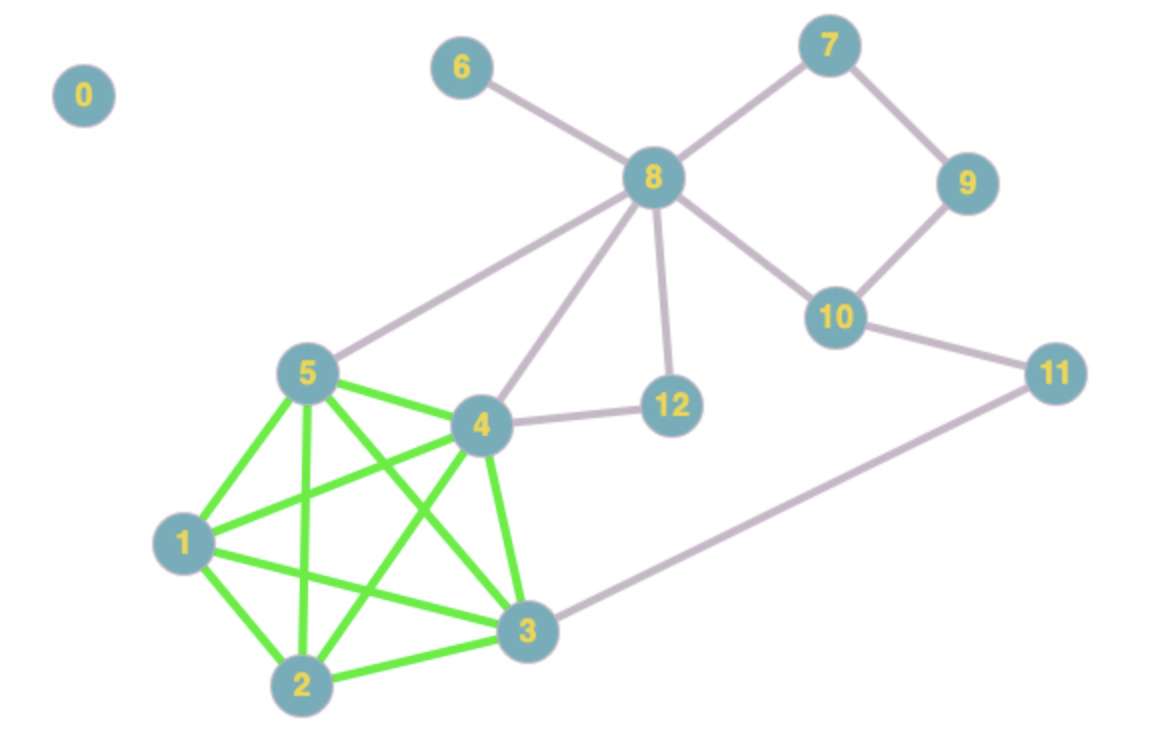
\includegraphics[width=0.7\textwidth]{img/connected_states.jpg}
\caption{Example of a graph of States}
\label{fig:connected_states}
\end{figure}

\subsection{Market}\label{section:market}
The market is an entity that will connect the agents. Its purpose is to allow interaction between agents of different States. It has no real functionality besides serving as a layer betwixt our agents and making sure both of them are allowed to exchange according to the rules that we have previously defined (sufficient stocks and money and connected States).

\subsection{World}\label{section:world}
After describing all our models, we eventually finish with the one that will encompass them all: the World. The purpose of this model will be to initialise all products, agents and States as well as let them be inter-connected through the Market.

The World will also handle the time step: a tick. Indeed, because computers are discrete machines, we have divide time into time steps (ticks). At each time step, our World will allow agents and States to perform actions such as producing, buying a product or collecting a tax.

However, as previously expressed, not all agents will perform an action at every tick. Only a certain percentage of the agents will do something: either produce, or buy, or do nothing (in case it has no money to either produce or buy, therefore it waits for someone to buy one of its products or for the State to give him an allowance). However, the action of selling may happen at anytime. This means that an consumer will be able to buy a product from a seller without waiting for him to also perform an action (otherwise, the system would be blocked very often).
This percentage value will be rather small due to the fact that a tick is something that will happen very often.

Finally, because our World contains all of the models we have defined (i.e. the products, the agents, the States and the Market), it will allow us to have an overview of all that is going on in our simulation. It will also be very useful in order to study the system and make some statistics.





\section{Implementation}\label{section:implementation}


This section will give an outlook of how the code implementation will be structured. However, one should note that the structure in this section is temporary and might be subject to changes when the code will be developed during the Master Thesis.

\subsection{Code}
The code will be written from scratch and take inspiration from the code already written by Nicolas Bernier in Java for his master thesis titled \textquote{Comparison between a competitive and a redistributive market economy using computer simulation} \cite{nicolasbernier}.

It will be written in Java following the Object-Oriented paradigm which suits our simulation the best because of the different models that we have described earlier. Python3 is not excluded yet, however Java will be preferred because an agent-based simulation is a very power consuming task best suited for strongly typed and compiled languages such as Java (whose main paradigm is based on OOP additionally).

\subsection{GUI and visualisation}
A Graphical User Interface (GUI) will be implemented in order to let the user tweak all of the available parameters (number of products, agents, States, clusters, money from start, and so on). This will be a more user-friendly way than putting these parameters in a file. However this "advanced user" feature will also be available in the form of a configuration file (such as an XML or a JSON file) which would be more handy for advanced user who do not want to bother with a GUI.

Furthermore, another module will be developed to picture the system. This module will create different statistical graphs based on the simulation (for example the Gini coefficient measuring the wealth distribution in a system and the inequalities, the amount of money in the Market at each time step, etc.). It will allow us to study the different questions we have asked ourselves in the section regarding the objectives (\ref{section:motivation_objectives}) and also see the importance of the parameters and how they can change the result of a simulation.

\subsection{Class diagram}

Finally, a temporary class diagram is presented in order to better visualise the interactions between the different models. This class diagram is partially based on the one made by Hugues Bersini in its 2012 publication titled \textquote{UML for ABM} \cite{umbforabm} but with adjustments to fit the model we have previously described in section~\ref{section:models}. The class diagram is depicted in Figure~\ref{fig:class_diagram}.


    \begin{figure}[H]
        \centering
        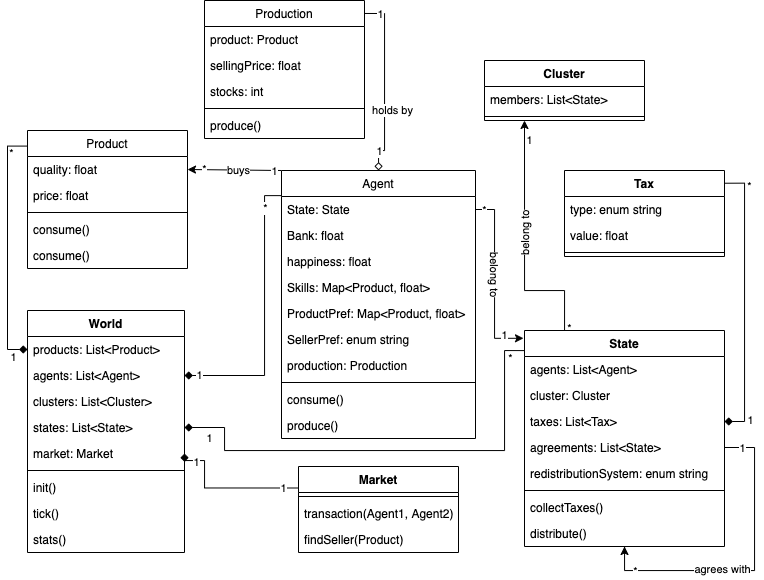
\includegraphics[width=1\textwidth]{img/class_diagram.png}
        \caption{Class diagram of the models}
        \label{fig:class_diagram}
    \end{figure}
